% diagrams/english/helado.tex -- el helado de Amy, para "Read and
% colour": el cucurucho (con su cuadrícula de barquillo), tres bolas una
% encima de otra y una cereza con su rabito.
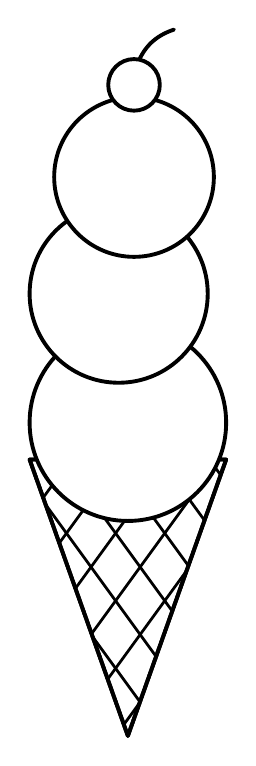
\begin{tikzpicture}[line width=1.4pt, line cap=round, line join=round, scale=0.78]
  % el cucurucho y su cuadrícula
  \filldraw[fill=white] (-1.6,4.5) -- (1.6,4.5) -- (0,0) -- cycle;
  \begin{scope}
    \clip (-1.6,4.5) -- (1.6,4.5) -- (0,0) -- cycle;
    \foreach \d in {-3,-2.2,...,3} {
      \draw[line width=1pt] (\d-2,0) -- (\d+2,5.5);
      \draw[line width=1pt] (\d+2,0) -- (\d-2,5.5);
    }
  \end{scope}
  \draw (-1.6,4.5) -- (1.6,4.5) -- (0,0) -- cycle;
  % las tres bolas, de abajo arriba
  \filldraw[fill=white] (0,5.1) circle (1.6);
  \filldraw[fill=white] (-0.15,7.2) circle (1.45);
  \filldraw[fill=white] (0.1,9.1) circle (1.3);
  % la cereza
  \draw (0.1,10.75) .. controls (0.2,11.2) and (0.45,11.4) .. (0.75,11.5);
  \filldraw[fill=white] (0.1,10.6) circle (0.42);
\end{tikzpicture}
